\label{Introduction}
% ---------------------------------------------------
\section{Background}
% \begin{enumerate}
%     \item Ligaments guide and restrict joint motion
%     \item Ligament properties influence knee joint behavior
%     \begin{enumerate}
%         \item Joint mechanics are sensitive to ligament slack length/prestrain
%     \end{enumerate}
%     \item Computer models are used to predict joint behavior
%     \begin{enumerate}
%         \item For intact joints and surgically repaired joints
%         \item Ligament representation varies between models
%     \end{enumerate}
%     \item Regardless of ligament representation, inverse modeling has been used to estimate ligament properties
%     \begin{enumerate}
%         \item Requires two components (1) Experimental testing (2) Joint model
%         \item Simulated experiment is used to iteratively change ligament properties until the computer model's predicted measurements match the experimental measurements
%         \item Ligament properties show large variability between specimens and experiements
%     \end{enumerate}
%     \item Ligament representation varies between models
%     \begin{enumerate}
%         \item Springs have been used to model joint level behavior
%         \item Solid continuum has been used to model joint level behavior as well as specific ligament behavior, however it is computationally expensive, which limits the possibilities for inverse modeling.
%     \end{enumerate}
% \end{enumerate}
%[Ligaments are important to joint function] 
Ligaments and articular contact define the limits of passive joint motion. Understanding the the forces acting across the knee and the resulting joint motion is important when assessing the causes and treatment of knee pathology \citep{thelen_co-simulation_2014} (\texthl{find better citation}).

%[The knee model's kinetics and contact mechanics are affected by ligament properties] 
Studies have shown that variations in ligament properties can affect the knee's kinematics and contact mechanics under simulated passive \citep{baldwin_efficient_2009,dhaher_effect_2010} and dynamic \citep{smith_influence_2016-1} joint loading.

%[Computational knee models are used to evaluate different knee treatments and pathology]

%[Computational models represent ligaments as nonlinear springs or an anisotropic continuum.] 
Computational knee models can use different representations of ligaments (\autoref{fig:continuumSpringAcl}), however there are few studies that evaluate the effects of ligament representation on the model's performance, and improvements can be made to the studies that have addressed this topic. \cite{beidokhti_influence_2017} used inverse modeling to generate comparable spring and continuum ligament models. The two types of models were considered equivalent if they yielded joint forces that were similar to experimentally measured values, however it was not shown that the spring and continuum ligament models yielded similar ligament forces under the same loading. Additionally, the prestrain definition may not be equivalent between the spring and continuum ligament representations. Conversely, \cite{orozco_effect_2018} applied similar prestrain to their spring and continuum ligament models, however prestrain was uniformly applied throughout each ligament. Joint mechanics have been shown to be sensitive to ligament prestrain \citep{baldwin_efficient_2009}, and experimental studies have shown that prestrain is not uniform throughout a ligament \citep{hull_strain_1996,gardiner_strain_2001}.

\begin{figure}
    \centering
    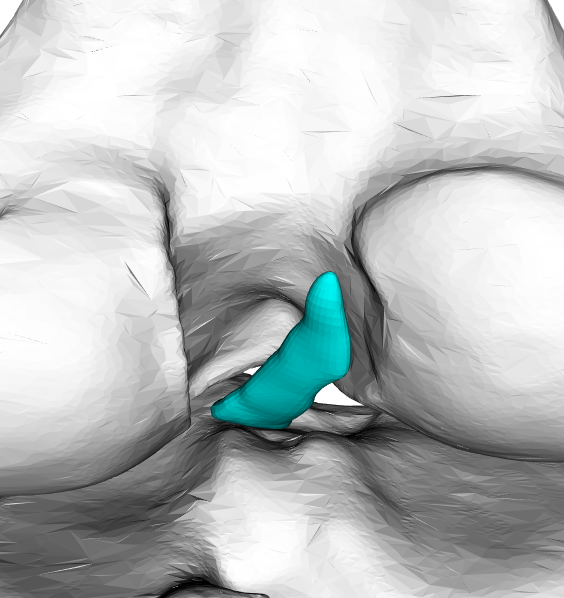
\includegraphics[width=0.35\linewidth]{../img/Knee_ACL_Close.png}
    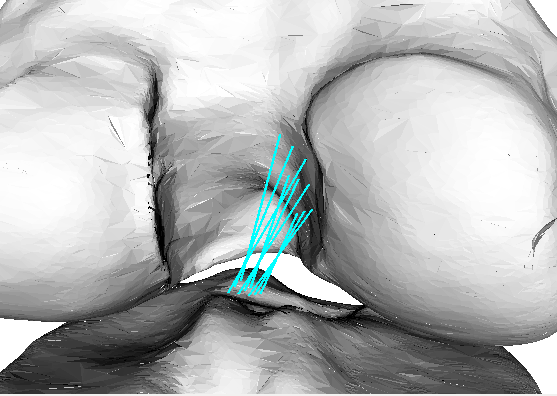
\includegraphics[width=0.35\linewidth]{../img/Knee_ACL_Springs_Close.png}
    \caption{A comparison of the anterior cruciate ligament (ACL) modeled as a (left) continuum and (right) a bundle of springs.}
    \label{fig:continuumSpringAcl}
\end{figure}

%[Prestrain can be assigned uniformly or nonuniformly across a continuum or spring model. Nonuniform continuum models assign prestrain directly from experimental data, where spring models have estimated prestrain with an inverse modeling scheme.] 
Nonhomogeneous prestrain can be assigned to spring and continuum ligament representations. Inverse modeling has been used to estimate specimen-specific ligament properties (including nonhomogeneous prestrain) for knee models that represent ligaments as springs \citep{blankevoort_validation_1996,baldwin_efficient_2009,ewing_estimating_2015,harris_combined_2016}. With the exception of \cite{gardiner_subject-specific_2003}, specimen-specific nonhomogeneous prestrain is not utilized in continuum ligament models. Literature is used to define prestrain values \citep{pena_three-dimensional_2006,dhaher_effect_2010}, which are derived from a combination of experimental studies and results of inverse modeling studies that utilize spring ligament models.

%[Prestrain in a continuum model could be informed with a corresponding calibrated spring model.]
A calibrated knee model that represents ligaments as springs could be used to estimate specimen-specific nonhomogeneous prestrain in continuum representations of ligaments. \cite{lu_computational_2007} estimated the prestrain in blood vessels using an inverse elastostatics approach, where the deformed state of the geometry and forces were known, and the stress-free shape of the geometry was estimated. 

% ---------------------------------------------------
\section{Overview}
%[Research questions and objectices: The purpose of this work is to develop an approach to defining ligament prestrain in a continuum ligament model.] 
The overall purpose of this work is to (1) develop an approach to estimating specimen-specific nonhomogeneous prestrain in ligaments that are represented as a continuum and (2) compare the performance of the continuum ligament representation to an equivalent spring ligament representation.

%[Approaches: ]
This approach assumes that the calibrated spring ligament model recreates the ligament's forces at a given joint position. These loading data could be used to define the boundary conditions for a inverse elastostatics analysis of a ligament. \cite{lu_computational_2007} used this approach to estimate the prestrain in blood vessels, where 

\begin{figure}
    \centering
    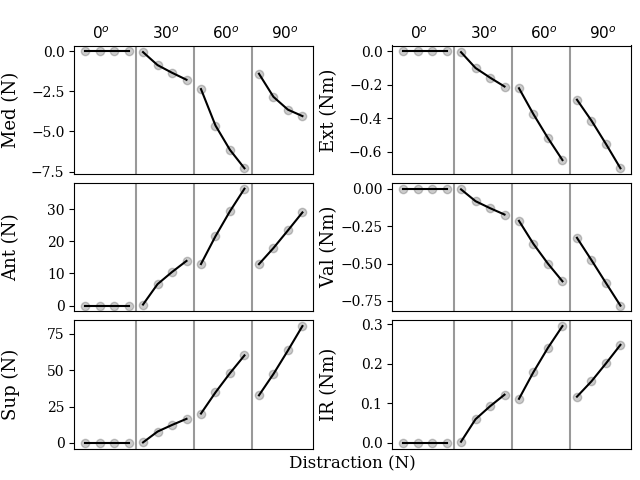
\includegraphics[width=0.75\linewidth]{../img/Spec1_Distraction_alPCL_Forces.png}
    \caption{An example of the forces and moments that the alPCL exerts on the tibia at four points throughout a distraction test at 0\textsuperscript{o}, 30\textsuperscript{o}, 60\textsuperscript{o}, 90\textsuperscript{o} flexion.}
    \label{fig:alPclForce}
\end{figure}

Ligaments are commonly represented as bundles of nonlinear uniaxial springs \citep{blankevoort_validation_1996,baldwin_efficient_2009,ewing_estimating_2015}, or as a solid continuum \citep{gardiner_subject-specific_2003,pena_three-dimensional_2006,dhaher_effect_2010} (\autoref{fig:continuumSpringAcl}). Joint mechanics have been shown to be sensitive to ligament prestrain \citep{baldwin_efficient_2009}, and experimental studies have shown that prestrain is not uniform throughout a ligament \citep{hull_strain_1996,gardiner_strain_2001}. Studies that utilize spring ligament representations can simulate nonhomogeneous prestrain in a ligament by varying the prestrain in each spring that composes a specific ligament. Studies that utilize continuum ligament representations either apply uniform prestrain \citep{limbert_three-dimensional_2004,song_three-dimensional_2004,beidokhti_influence_2017}, or apply nonhomogeneous prestrain based on values reported in the literature \citep{pena_three-dimensional_2006,dhaher_effect_2010}, where prestrains are derived from a combination of experimental studies and results of inverse modeling studies that utilize spring ligament models.

Representing ligaments as springs allows for the prediction of joint level mechanics such as kinematics \citep{weiss_computational_2001}. Ligaments are normally modeled as bundles of springs, where each spring's insertion lies within the insertion area of the ligament. Nonhomogenous prestrain can be simulated by varying the prestrain assigned to each spring in a ligament. Due to their computational efficiency, spring ligament models are used in inverse modeling studies to estimate ligament properties, including as prestrain \citep{blankevoort_validation_1996,baldwin_dynamic_2012,ewing_estimating_2015,harris_combined_2016}.

Specimen-specific knee models are defined with geometry derived from MR images, and ligament material properties are normally estimated with inverse modeling \citep{blankevoort_validation_1996,baldwin_dynamic_2012,ewing_estimating_2015,harris_combined_2016}. These models normally utilize spring representations of ligaments because they have been shown to allow for the prediction of joint kinematics \citep{weiss_computational_2001}, and they are computationally efficient. A recent study by \cite{beidokhti_influence_2017} compared the effects of ligament representation on a knee model's predicted joint mechanics. That study used inverse modeling to estimate ligament properties for two different knee models, one with spring ligament representations, and the other with continuum ligament representations. 

A recent study compared joint mechanics between knees modeled with spring and continuum ligament representations for passive loading \citep{beidokhti_influence_2017}. This study evaluated the effects of ligament representation on joint mechanics, however the prestrain definition between two types of ligament representations may not be equivalent. \cite{beidokhti_influence_2017} used inverse modeling to generate comparable spring and continuum joint level models. Multiple springs were used to model each of the cruciate and collateral ligaments, where each spring can have a unique prestrain. Conversely, each continuum ligament was modeled as one body that had prestrain uniformly applied throughout. \cite{gardiner_subject-specific_2003} showed that an nonhomogenous prestrain can have an impact on the strain distribution within a ligament under load. 

%[The approach will use inverse modeling to first calibrate a spring model.]

%[Force results from the spring model will be used as boundary conditions for the]

% ---------------------------------------------------
\subsection{Specific Aims}
% ........................
\subsubsection{Distraction Experiment}
Distraction testing will provide a novel data set that is suitable to estimate ligament properties with an inverse modeling scheme. Two knee specimens will be prepared and MR imaged to facilitate model development. The specimens will be tested with common laxity-style loads, and with novel laxity-style distraction loads. The applied joint forces and the corresponding joint kinematics will be measured throughout testing. The MR imaging will provide the data necessary to create specimen-specific geometry, and the measurements taken during preparation and testing will provide the data necessary for estimation of ligament properties with inverse modeling.

\emph{Status:} Complete

\emph{Contribution:} Data necessary to create specimen-specific models and simulate the experimental tests.
% ........................
\subsubsection{Inverse Modeling with Distraction Testing}
Inverse modeling will be used to estimate specimen-specific ligament slack-length using data from distraction testing. Use of an experimentally novel joint state and joint loads allows for joint contact to be neglected in the computational model, and may focus the joint's force-displacement behavior on the ligaments. Neglecting contact enables the use of a computationally efficient forward kinematics model, which is used in an inverse modeling scheme to estimate ligament slack-length. This will provide a calibrated model that recreates the experimental conditions. 

\emph{Status:} Complete

\emph{Contribution:} A novel approach to using inverse modeling to estimate ligament properties.
% ........................
\subsubsection{Ligament Recruitment Probability}

\emph{Status:}

\emph{Contribution:}
% ........................
\subsubsection{Continuum Ligament Prestrain}

\emph{Status:}

\emph{Contribution:}